\documentclass[conference]{../IEEEtran/IEEEtran}

\usepackage{amsmath}
\usepackage{array}
\usepackage{booktabs}
\usepackage{graphicx}
\usepackage{url}
\usepackage[hidelinks,breaklinks=true]{hyperref}

\graphicspath{{../diagrams/}{../pictures/}}
\renewcommand{\ttdefault}{cmtt}
\urlstyle{same}
\Urlmuskip=0mu plus 1mu\relax
\setlength{\textfloatsep}{7pt plus 1pt minus 2pt}
\setlength{\floatsep}{7pt plus 1pt minus 2pt}
\setlength{\intextsep}{7pt plus 1pt minus 2pt}
\setlength{\abovecaptionskip}{3pt}
\setlength{\belowcaptionskip}{-2pt}

\begin{document}

\title{OKX Pulse: Real-Time HFT Signal Inference with Executable-PnL Labels}

\author{
    \IEEEauthorblockN{Tuan Minh Pham}
    \IEEEauthorblockA{
        Course Project Report\\
        COSC6376 - Cloud Computing\\
        Email: \textit{tmpham42@cougarnet.uh.edu}
    }
}

\maketitle
\raggedbottom

\begin{abstract}
    This report describes OKX Pulse, a course project for real-time trading signal inference on OKX market data. The system uses a C++ runtime, a Python machine-learning pipeline, an Electron interface, and Docker/AWS deployment files. The main idea is to train and test signals with executable bid/ask profit-and-loss labels, not only future price direction. This target is harder because a trade must cover the spread before it can make profit. The system shows a local gRPC loop between the C++ runtime and the Python inference service. It also compares XGBoost and LightGBM on a dataset where most labels are neutral, and compares ECS on EC2 with ECS on Fargate. The final test results did not give positive executable PnL. However, the results show that order-book and trade-flow features still have useful information. More work is needed on labels, feature parity, and threshold choice.
\end{abstract}

\begin{IEEEkeywords}
    high-frequency trading, market microstructure, order book, machine learning, gRPC, ECS, Fargate, OKX
\end{IEEEkeywords}

\section{Introduction}

High-frequency trading systems are hard to evaluate with simple price-direction labels. A model can predict a small future mid-price move correctly, but the trade can still lose money after the spread, fees, latency, and execution limits. OKX Pulse handles this problem by using executable trading edge. The project does not only ask whether the future price goes up or down. It asks whether buying at the current ask and selling at a future bid, or selling at the current bid and buying back at a future ask, would give positive PnL.

The project has three goals. First, it builds a real-time service architecture for OKX market data and gRPC streaming~\cite{okx-docs,grpc-docs}. Second, it keeps online C++ features aligned with offline Python training features. This helps reduce train/serve drift. Third, it prepares local container and AWS deployment files, then compares ECS on EC2 with ECS on Fargate.

\section{System Architecture}

The system has two main paths: online runtime and offline training. The online path is latency-sensitive, so it stays local and uses C++ for market data, feature building, strategy logic, and paper trading~\cite{binance-quant-trader}. Python is used for model serving and offline machine-learning work.

\begin{figure}[!t]
    \centering
    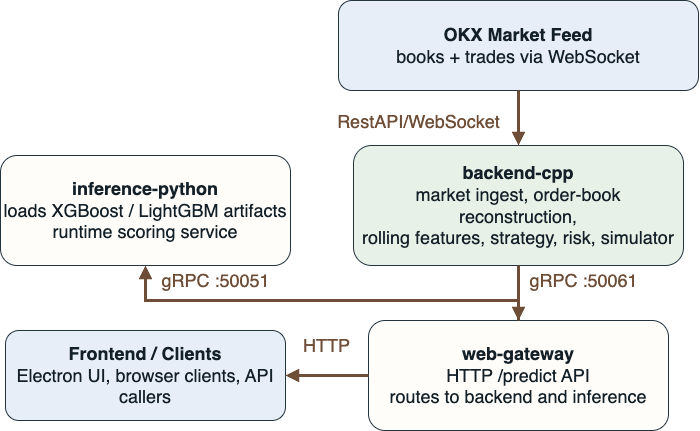
\includegraphics[width=\linewidth]{runtime_architecture.drawio.png}
    \caption{Runtime architecture. The C++ service reads OKX market data, builds features, streams data over gRPC, and calls the Python inference service.}
    \label{fig:runtime}
\end{figure}

\subsection{Online Runtime}

The online runtime starts from OKX WebSocket data. The C++ backend reads book and trade updates, keeps rolling feature state, can write feature rows to CSV, and publishes a \texttt{MarketData} gRPC stream on port 50051. The Python inference service exposes a \texttt{PredictionService} gRPC endpoint on port 50061. Runtime messages can also include prediction fields such as model name, signal, return estimate, price estimate, and detail text.

\begin{table}[!t]
    \caption{Runtime services.}
    \label{tab:services}
    \centering
    \small
    \begin{tabular}{@{}p{0.36\linewidth}p{0.14\linewidth}p{0.38\linewidth}@{}}
        \toprule
        \textbf{Service}          & \textbf{Stack} & \textbf{Role}                  \\
        \midrule
        \texttt{backend-cpp}      &
        C++                       &
        OKX ingest, feature generation, strategy, paper trading, and gRPC streaming \\
        \texttt{inference-python} &
        Python                    &
        Model loading and prediction service                                        \\
        \texttt{web-gateway}      &
        Node.js                   &
        HTTP routing for clients and UI access                                      \\
        \bottomrule
    \end{tabular}
\end{table}

\subsection{Offline Training Path}

The offline path converts captured or historical market data into feature rows. It then builds labels from future executable PnL, trains models, tests thresholded trading results, and stores model files. This separation makes experiments easier while keeping a clear link between training columns and online feature names.

\section{Data Contracts}

The repository uses two main data contracts. The live service contract is defined in \texttt{backend/proto/market\_data.proto}. It includes a streaming \texttt{MarketData.Subscribe} interface and a request/response \texttt{PredictionService.Predict} interface. The offline contract is a normalized CSV feature table. The runtime creates this table, and the Python training pipeline uses it.

The most important rule is feature parity. Online C++ feature names and offline Python training columns must stay aligned. If they do not match, train/serve drift can happen even when the model and service code run correctly.

\section{Feature Engineering and Labels}

The project uses market microstructure features in four groups: price state, order-book pressure, trade flow, and short-horizon changes. Price-state features include mid price, spread, relative spread, and microprice. Order-book features include level-1 and five-level imbalance. Trade-flow features include recent trade volume, trade imbalance, and trade VWAP. Short-horizon features track recent changes in mid price, spread, and book imbalance.

\begin{figure}[!t]
    \centering
    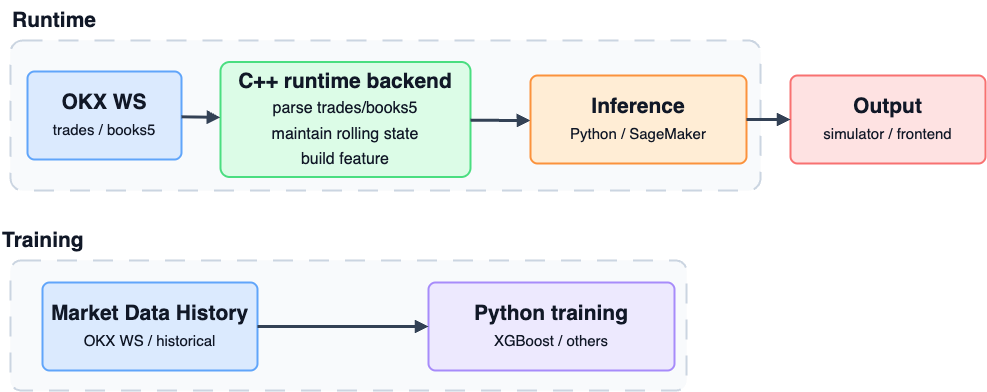
\includegraphics[width=\linewidth]{flowchart.drawio.png}
    \caption{Feature and label-building flow. Book and trade data are converted into features, then future bid/ask values are used to build executable-PnL labels.}
    \label{fig:flow}
\end{figure}

\subsection{Executable-PnL Label}

For a prediction horizon $H$, the project checks whether a crossed-spread trade would make profit. A long trade buys at the current ask and exits at the future bid:

\begin{equation}
    \mathrm{buy\_pnl}_H = \mathrm{bid}_{H} - \mathrm{ask}_{now}.
\end{equation}

A short trade sells at the current bid and exits at the future ask:

\begin{equation}
    \mathrm{sell\_pnl}_H = \mathrm{bid}_{now} - \mathrm{ask}_{H}.
\end{equation}

The class label is:

\begin{equation}
    \mathrm{label}_H =
    \begin{cases}
        1,  &
        \begin{aligned}[t]
            \mathrm{buy\_pnl}_H  &> \epsilon \ \mathrm{and} \\
            \mathrm{buy\_pnl}_H  &> \mathrm{sell\_pnl}_H
        \end{aligned} \\
        -1, &
        \begin{aligned}[t]
            \mathrm{sell\_pnl}_H &> \epsilon \ \mathrm{and} \\
            \mathrm{sell\_pnl}_H &> \mathrm{buy\_pnl}_H
        \end{aligned} \\
        0,  & \mathrm{otherwise}.
    \end{cases}
\end{equation}

Here, label 1 means executable long edge. Label -1 means executable short edge. Label 0 means no clear edge. This target is stricter than raw direction classification because it includes the spread cost.

\section{Modeling Results}

The ML pipeline was rechecked from the saved dataset and evaluation files. The final comparison uses 86,399 rows and 43 columns. The data is split by time into 69,119 training rows and 17,280 testing rows. The training part is also split into 55,296 fitting rows and 13,823 calibration rows. The model uses 20 feature columns and predicts signed executable return. Most labels are neutral. This is expected because the label requires executable edge, not only a small price move.

The archive builder requested several days of OKX data, but the effective timestamps in this run came from April 12, 2026. Because of this, the result should be read as a one-day experiment. More days are still needed before the model can be called robust.

\begin{table}[!t]
    \caption{Dataset snapshot.}
    \label{tab:dataset}
    \centering
    \small
    \begin{tabular}{@{}lr@{}}
        \toprule
        \textbf{Metric} & \textbf{Value}      \\
        \midrule
        Rows            & 86,399              \\
        Columns         & 43                  \\
        Train rows      & 69,119              \\
        Test rows       & 17,280              \\
        Split           & chronological 80/20 \\
        \bottomrule
    \end{tabular}
\end{table}

\begin{table}[!t]
    \caption{Executable-label distribution.}
    \label{tab:labels}
    \centering
    \small
    \begin{tabular}{@{}lrr@{}}
        \toprule
        \textbf{Label} & \textbf{Train} & \textbf{Test} \\
        \midrule
        Down           & 6,341          & 2,159         \\
        Neutral        & 56,176         & 13,226        \\
        Up             & 6,602          & 1,895         \\
        \bottomrule
    \end{tabular}
\end{table}

\begin{figure}[!t]
    \centering
    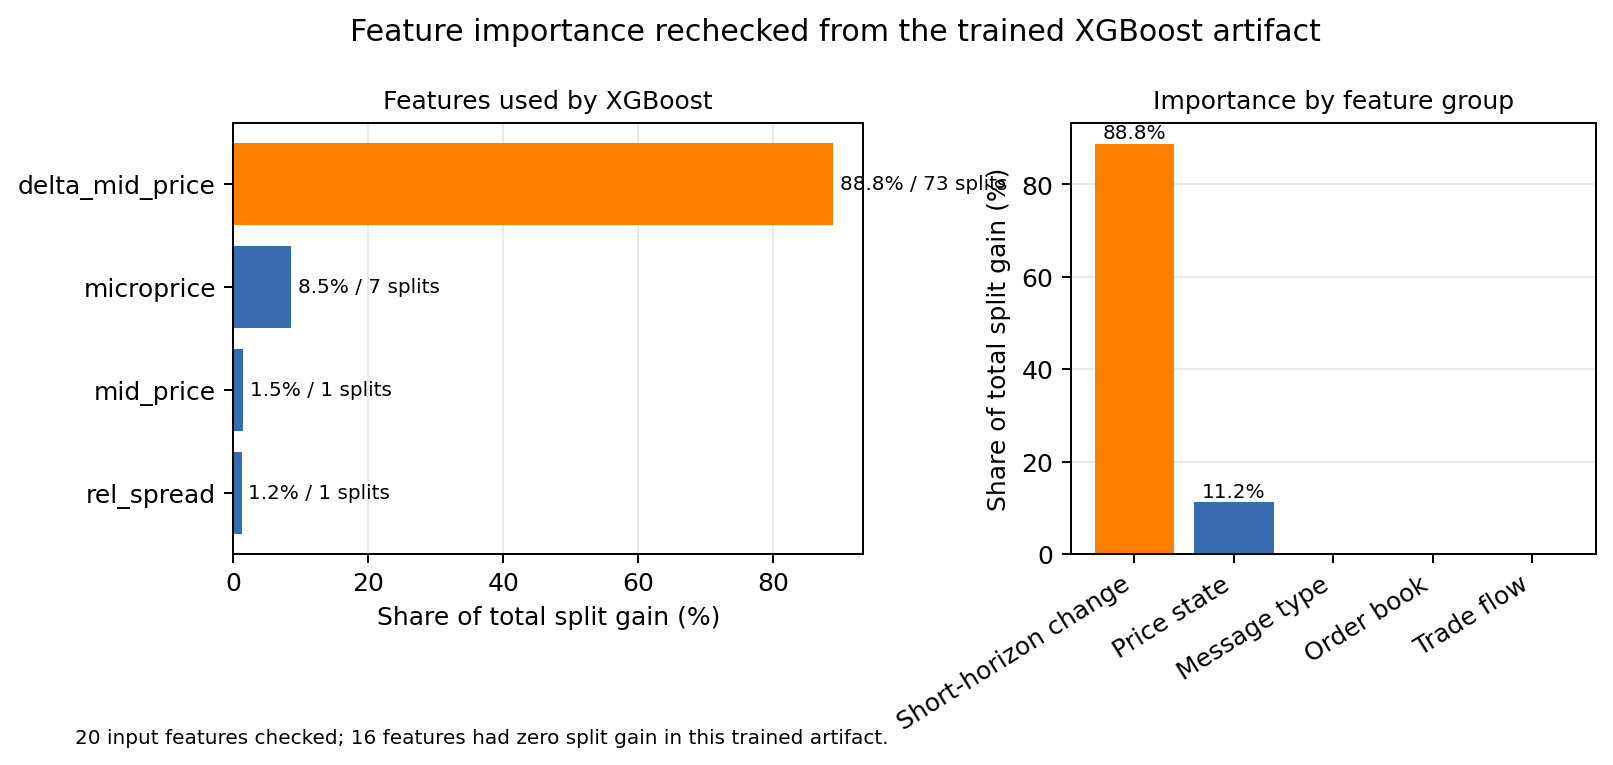
\includegraphics[width=0.96\linewidth]{feature_importance.png}
    \caption{Feature importance rechecked from the trained XGBoost artifact. Most split gain came from \texttt{delta\_mid\_price} and price-state features in this run.}
    \label{fig:importance}
\end{figure}

The feature-importance check gives an important warning. The trained XGBoost model does not use all feature groups equally. In this run, 16 of the 20 input features have zero split gain. Most useful signal comes from short-horizon mid-price change and price-state features. This means the current dataset is still too small or too narrow for many depth and trade-flow features to help much.

The final held-out comparison uses XGBoost and LightGBM~\cite{xgboost,lightgbm}. The two models have similar error size, but XGBoost has higher correlation with the signed executable return. Table~\ref{tab:model_quality} shows the model quality on the test split. MAE and RMSE are shown in basis points.

\begin{table}[!t]
    \caption{Return prediction quality on the test split.}
    \label{tab:model_quality}
    \centering
    \small
    \begin{tabular}{@{}lrrrr@{}}
        \toprule
        \textbf{Model} & \textbf{MAE} & \textbf{RMSE} & \textbf{Corr.} & \textbf{Dir. Acc.} \\
        \midrule
        XGBoost  & 0.311 & 0.670 & 0.233 & 23.47\% \\
        LightGBM & 0.318 & 0.666 & 0.205 & 23.48\% \\
        \bottomrule
    \end{tabular}
\end{table}

Neither model reaches positive executable PnL on the test split after threshold selection. XGBoost makes 691 trades at a 0.3 bps threshold with -295.6 PnL per BTC and a 29.23\% win rate. LightGBM makes 248 trades at a 0.5 bps threshold with -604.7 PnL per BTC and a 23.79\% win rate.

\begin{table}[!t]
    \caption{Held-out executable-PnL model results.}
    \label{tab:results}
    \centering
    \scriptsize
    \setlength{\tabcolsep}{2.2pt}
    \begin{tabular}{@{}lrrrrrr@{}}
        \toprule
        \textbf{Model} & \textbf{Th.} & \textbf{Trades} & \textbf{Cov.} & \textbf{PnL/BTC} & \textbf{PnL/\$5k} & \textbf{Win} \\
        \midrule
        XGBoost  & 0.3 bps & 691 & 3.999\% & -295.6 & -20.76 & 29.23\% \\
        LightGBM & 0.5 bps & 248 & 1.435\% & -604.7 & -42.53 & 23.79\% \\
        \bottomrule
    \end{tabular}
\end{table}

\begin{figure}[!t]
    \centering
    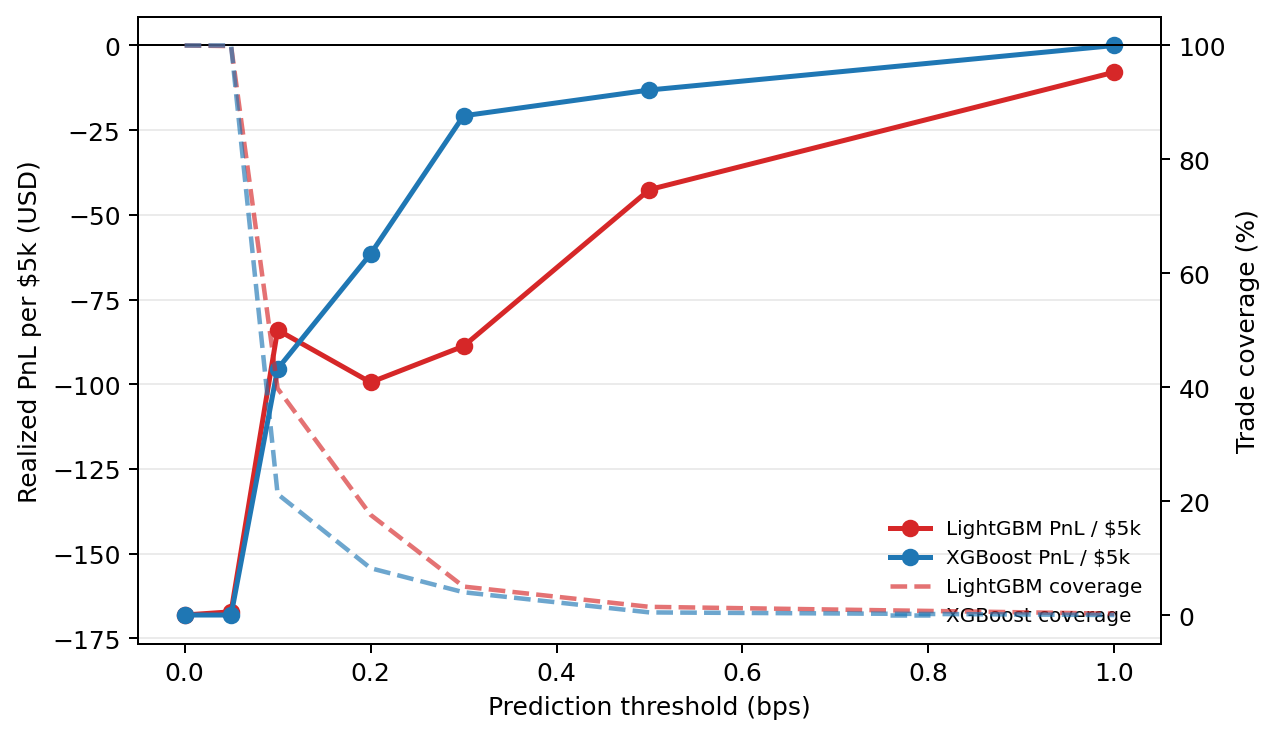
\includegraphics[width=0.96\linewidth]{threshold_sweep.png}
    \caption{Threshold sweep on the held-out test split. Higher thresholds reduce trade coverage and reduce the loss, but they do not make the strategy profitable.}
    \label{fig:threshold}
\end{figure}

The threshold sweep gives more useful information than one final number. With no threshold, both models trade almost every row and lose about \$168 per \$5k notional. A higher threshold reduces the number of trades and lowers drawdown. For XGBoost, the selected 0.3 bps threshold gives 4.00\% coverage and about \$33.40 maximum drawdown per \$5k. For LightGBM, the selected 0.5 bps threshold gives 1.44\% coverage and about \$47.50 maximum drawdown per \$5k.

These results are still useful. They show that the feature set has some structure, but the current signal is not strong enough to beat spread and execution costs. The expected PnL from the model is positive, but the realized PnL is negative. This means calibration is not reliable enough yet. The safest runtime choice is shadow mode, where predictions are logged and watched but not used for live trading.

\section{Deployment Evaluation}

The deployment files package three services: \texttt{backend-cpp}, \texttt{inference-python}, and \texttt{web-gateway}. The local container runtime uses Docker Compose. The AWS files include ECS task definitions, ECS service templates, EC2 scripts, and Terraform notes~\cite{aws-ecs}.

\begin{figure}[!t]
    \centering
    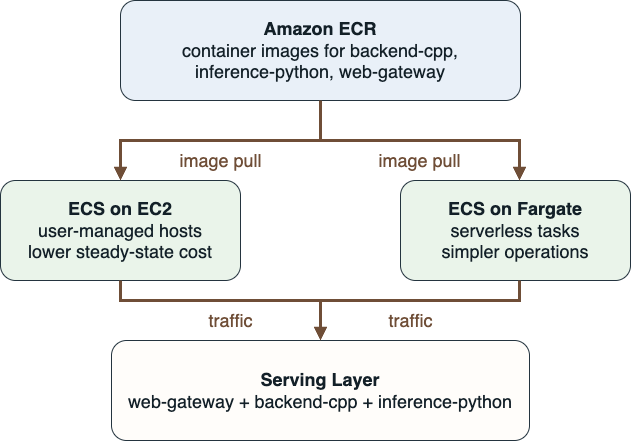
\includegraphics[width=0.84\linewidth]{aws_deployment_containers.drawio.png}
    \caption{Container deployment view for the runtime services.}
    \label{fig:deployment}
\end{figure}

The recommended deployment is ECS on EC2 for always-on serving. It gives lower steady-state cost and more host control. Fargate is still useful when simple operation matters more than cost. The project estimate gives about \$36.79 per month for three \texttt{t4g.small} EC2 nodes. The same three services on Fargate cost about \$90.10 per month, plus about \$1.20 per month for 11.9598 GiB of ECR storage.

\section{Lessons Learned}

The most important lesson is that label design has a large effect on trading results. Direction classification is easier, but executable PnL labels match the real decision better. The second lesson is that train/serve feature parity must be treated as a system contract, not only as a notebook detail. The third lesson is that deployment should match runtime needs. Cloud infrastructure is useful for packaging, service management, observability, and reproducibility. However, the live inference hop should stay local and internal for the main trading loop.

\section{Conclusion}

OKX Pulse shows a real-time HFT signal inference platform with C++ market-data processing, Python model serving, gRPC contracts, Electron UI support, and AWS container deployment files. The final models do not produce positive held-out executable PnL. However, the system gives a clear base for more work on data quality, feature parity, thresholding, and model choice. ECS on EC2 is the better option for cost-efficient always-on deployment. Fargate is better when lower operation work is more important. Executable-PnL labels should continue to be used for realistic signal testing.

\begin{thebibliography}{1}

    \bibitem{okx-docs}
    OKX, ``API Documentation v5 and Historical Data.'' [Online]. Available: \href{https://www.okx.com/docs-v5/en/}{API docs}; \href{https://www.okx.com/historical-data}{historical data}. Accessed May 7, 2026.

    \bibitem{grpc-docs}
    gRPC Authors, ``Documentation.'' [Online]. Available: \href{https://grpc.io/docs/}{grpc.io/docs}. Accessed May 7, 2026.

    \bibitem{binance-quant-trader}
    VinaDevs, ``BinanceQuantTrader.'' [Online]. Available: \href{https://github.com/vinadevs/BinanceQuantTrader}{GitHub repo}. Accessed May 7, 2026.

    \bibitem{xgboost}
    T. Chen and C. Guestrin, ``XGBoost: A scalable tree boosting system,'' in \emph{Proc. KDD}, 2016, pp. 785--794, doi: \href{https://doi.org/10.1145/2939672.2939785}{10.1145/2939672.2939785}.

    \bibitem{lightgbm}
    G. Ke \emph{et al.}, ``LightGBM: A highly efficient gradient boosting decision tree,'' in \emph{NeurIPS}, vol. 30, 2017. [Online]. Available: \href{https://papers.nips.cc/paper/6907-lightgbm-a-highly-efficient-gradient-boosting-decision-tree}{NeurIPS page}.

    \bibitem{aws-ecs}
    AWS, ``ECS and Fargate Documentation.'' [Online]. Available: \href{https://aws.amazon.com/documentation-overview/ecs/}{ECS docs}; \href{https://aws.amazon.com/documentation-overview/fargate/}{Fargate docs}. Accessed May 7, 2026.

\end{thebibliography}

\end{document}
